\section{Движение тела, брошенного под углом к горизонту}

\introProblems

\begin{ex} %Сив21
Из артиллерийского орудия произведен выстрел под углом $\varphi$ к горизонту. Величина начальной скорости снаряда $v_0$. Исследовать аналитически движение снаряда, пренебрегая сопротивлением воздуха полету снаряда и кривизной поверхности Земли. Найденные зависимости изобразить графически. Найти: 1) вертикальную и горизонтальную компоненты вектора скорости $\vec{v}$ и абсолютную величину скорости как функцию времени; 2) время $Т$ полета снаряда от орудия до падения на землю; 3) зависимость от времени угла $\alpha$ между вектором скорости снаряда и горизонтом; 4) декартовы координаты (ось $X$ — горизонтальное направление, ось $Y$ — вертикальное направление) снаряда как функции времени; 5) уравнение траектории снаряда $y = f(x)$ (построить согласно этому уравнению траекторию полета снаряда); 6) максимальную высоту $H_{max}$ полета снаряда над землей; 7) горизонтальную дальность $L_{max}$ полета снаряда как функцию его начальной скорости и угла возвышения орудия; 8) При каком угле возвышения $\varphi^*$ дальность будет максимальной при заданной начальной скорости снаряда?
\begin{ans}
1) $v_x = v_0 \cos \varphi$, $v_y = v_0 \sin \varphi - gt$, $v = \sqrt{v_{0}^{2} + g^2 t^2 - 2v_{0}gt \sin \varphi}$; 2) $T = \frac{2v_{0}\sin \varphi}{g}$; 3) $ \tg \alpha = \tg \varphi - \frac{gt}{v_0 \cos \varphi}$; 4) $x = v_0 t \cos \varphi$, $y = v_0 t \sin \varphi - \frac{gt^2}{2}$; 5) $y = x \tg \varphi - \frac{gx^2}{2v_{0}^{2} \cos^2 \varphi} $; 6) $H_{\max} = \frac{v_{0}^{2} \sin^2 \varphi}{2g}$; 7) $L_{\max} = v_{0}^2 \sin 2 \varphi / g$; 8) $\varphi^{*} = 45^{\circ}$.
\end{ans}
\end{ex}	

\begin{ex} %Сив30
Самолет летит на высоте $h$ горизонтально по прямой со скоростью $v$. Летчик должен сбросить бомбу в цель, лежащую впереди самолета. Под каким углом $\alpha$ к вертикали он должен видеть цель в момент выпуска бомбы? Каково в этот момент расстояние $l$ от цели до точки, над которой находится самолет? Сопротивление воздуха движению бомбы не учитывать.
\begin{ans}
$\tg \alpha = v \sqrt{2/hg}$, $l = v \sqrt{2h/g}$.
\end{ans}
\end{ex}	

\begin{ex} %Иродов1.10
Два тела бросили одновременно из одной точки: одно — вертикально вверх, другое - под углом $\alpha = 60^{\circ}$ к горизонту. Начальная скорость каждого тела $v_0 = 25$ м/с. Найти расстояние между телами через $t = 1,70$ с.
\begin{ans}
$l = v_0 t \sqrt{2(1-\sin \alpha)} = 22$ м.
\end{ans}
\end{ex}	

\begin{ex} %Сив32
Цель, находящаяся на холме, видна с места расположения орудия под углом $\alpha$ к горизонту. Дистанция (расстояние по горизонтали от орудия до цели) равна $L$. Стрельба по цели производится при угле возвышения $\beta$. Определить начальную скорость $v_0$ снаряда, попадающего в цель. Сопротивление воздуха не учитывать.
\begin{ans}
$v_0 = \sqrt{\frac{lg \cos \alpha}{2 \cos \beta \sin \left( \beta - \alpha \right)}}$.
\end{ans}
\end{ex}

\qualProblems
\begin{ex} %Morin
Пуля вылетела горизонтально из ружья, одновременно с ней другая пуля начала падать вертикально с той же высоты. Какая пуля первой достигет земли, если пренебречь сопротивлением воздуха, кривизной поверхности Земли и т.д.).
\begin{ans}
Одновременно.
\end{ans}
\end{ex}

\begin{ex} %Марон
В каком случае выброшенная из вагона вещь долетит до земли раньше -- когда вагон покоится или когда он движется?
\begin{ans}
За одинаковое время.
\end{ans}
\end{ex}	

\begin{ex} %Morin
Камень брошен под углом к горизонту. Существует ли такое положение в процессе движения, в котором скорость перпендикулярна ускорению камня?
\begin{ans}
Верхняя точка траектории.
\end{ans}
\end{ex}	

\begin{ex} %Morin
Неопытный охотник бросает камень в обезьяну, сидящую на дереве высотой $H$ на расстоянии $L$ по горизонтали от охотника, при этом направляет вектор начальной скорости $v_0$ в местоположение обезьяны. В момент броска камня обезьяна отпускает руки и начинает свободно падать с дерева без начальной скорости. При каком условии камень может настичь обезьяну? 
\begin{ans}
$v_0 > \sqrt{\frac{g(H^2+L^2)}{2H}}$.
\end{ans}
\end{ex}	

\simpleProblems

\begin{ex} %Сив18
Какой начальной скоростью $v_0$ должна обладать сигнальная ракета, выпущенная из ракетницы под углом $45^{\circ}$ к горизонту, чтобы она вспыхнула в наивысшей точке своей траектории, если время горения запала ракеты 6 с? Сопротивление воздуха движению ракеты не учитывать.
\begin{ans}
$v_0 = 82$ м/с.
\end{ans}
\end{ex}	

\begin{ex} %ПодОл3-1
Точка движется согласно уравнениям: $x = 2t + 6, y = t^2$. Проходит ли ее траектория через точку $x = 10, y = 10$? Найдите величину и направление ускорения точки?
\begin{ans}
Нет, $a = 2$ м/с\textsuperscript{2}.
\end{ans}
\end{ex}	

\begin{ex} %Сив23
Из трех труб, расположенных на земле, с одинаковой скоростью бьют струи воды: под углом в $60^{\circ}$, $45^{\circ}$ и $30^{\circ}$ к горизонту. Найти отношение наибольших высот $H$ подъема струй воды, вытекающих из каждой трубы, и отношение дальностей падения $L$ воды на землю. Сопротивление воздуха движению водяных струй не учитывать.
\begin{ans}
$H_1 : H_2 : H_3 = 3 : 2 : 1$; $L_1 : L_2 : L_3 = \sqrt{3} : 2 : \sqrt{3}$.
\end{ans}
\end{ex}	

\begin{ex} %ПодОл3-5
Под каким углом к горизонту надо бросить камень, чтобы дальность его полета была втрое больше максимальной высоты подъема?
\begin{ans}
$55,1^{ \circ }$.
\end{ans}
\end{ex}	

\begin{ex} %Сив24
На какое максимальное расстояние $L$ можно бросить мяч в спортивном зале высотой 8 м, если мяч имеет начальную скорость 20 м/с? Какой угол $\varphi$ с полом зала должен в этом случае составлять вектор начальной скорости мяча? Считать, что высота начальной точки траектории мяча над полом мала по сравнению с высотой зала. Мяч во время полета не должен ударяться о потолок зала. Сопротивлением воздуха полету мяча пренебречь.
\begin{ans}
$L \approx 40$ м, $\varphi \approx 38^{\circ}40^\prime$.
\end{ans}
\end{ex}	

\begin{ex} %ПодОл3-8 
Камень бросили с крутого берега реки вверх под углом $30^{\circ}$ к горизонту со скоростью $v_0 = 10$ м/с. С какой скоростью он упал в воду, если время полета $t = 2$ с?
\begin{ans}
17 м/с.
\end{ans}
\end{ex}	

\begin{ex} %Сив32
Два шарика брошены с одинаковой скоростью $v_0$ с крыши под одинаковыми углами  $\theta$ один выше горизонта, другой ниже (рис. \ref{edgeClif2balls}). На каком расстоянии друг от друга шарики приземляться на поверхности земли.
\begin{ans}
$s = \frac{2 v_0^2 \cos \alpha \sin \alpha}{g}$.
\end{ans}
\end{ex}

\begin{figure}
\centering
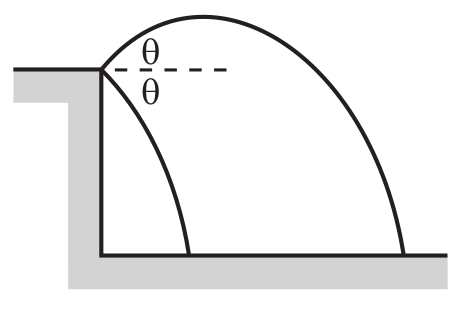
\includegraphics[width=0.4\textwidth]{edgeClif2balls.png}
\caption{}
\label{edgeClif2balls}
\end{figure}

\complexProblems

\begin{ex} %Иродов1.11
Два шарика бросили одновременно из одной точки в горизонтальном направлении в противоположные стороны со скоростями $v_1 = 3,0$ м/с и $v_2 = 4,0$ м/с. Найти расстояние между шариками в момент, когда их скорости окажутся взаимно перпендикулярными.
\begin{ans}
$l = (v_1 + v_2)\sqrt{v_1 v_2}/g = 2,5$ м.
\end{ans}
\end{ex}	

\begin{ex} %ПодОл3-13 
Утка летела по горизонтальной прямой с постоянной скоростью $u$. В нее бросил камень неопытный охотник, причем бросок был сделан без упреждения, т.е. в момент броска скорость камня $v$ была направлена как раз на утку под углом $\alpha$ к горизонту (рис. \ref{duckHunter}). На какой высоте летела утка, если камень все же попал в нее? С какой стороны камень ударил утку?

\begin{figure}
\centering
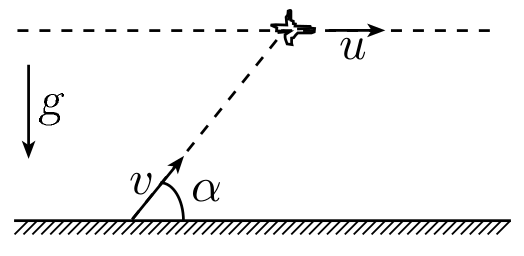
\includegraphics[width=0.4\textwidth]{duckHunter.png}
\caption{}
\label{duckHunter}
\end{figure}

\begin{ans}
$h = \frac{2u}{g}\left( v \cos \alpha - u \right) \tg^2 \alpha$.
\end{ans}
\end{ex}

\begin{ex} %Сив20
Шарик, которому сообщена горизонтальная скорость $v$, падает на горизонтальную плиту с высоты $h$. При каждом ударе о плиту вертикальная составляющая скорости уменьшается (отношение вертикальной составляющей скорости после удара к ее значению до удара
постоянно и равно $\alpha$). Определить, на каком расстоянии $х$ от места бросания отскоки шарика прекратятся. Считать, что трение отсутствует, так что горизонтальная составляющая скорости шарика $v$ не меняется
\begin{ans}
$x = v \sqrt{2h/g} \left( 1 + \alpha \right) / \left( 1 - \alpha \right)$.
\end{ans}
\end{ex}

\clearpage